\documentclass[journal=jpclcd,manuscript=article]{achemso}

\usepackage[version=3]{mhchem} % Formula subscripts using \ce{}
\usepackage[T1]{fontenc}       % Use modern font encodings

\newcommand*\mycommand[1]{\texttt{\emph{#1}}}

\author{Authors}
\altaffiliation{Huygens-Kamerlingh Onnes Laboratory, Leiden University, RA, Leiden, The Netherlands}
\email{corresponding_author@physics.leidenuniv.nl}
\title[]
{Electrochemsitry of single Azurin shows time variant turnovers}

\abbreviations{IR,NMR,UV}
\keywords{American Chemical Society, \LaTeX}

\begin{document}

%%%%%%%%%%%%%%%%%%%%%%%%%%%%%%%%%%%%%%%%%%%%%%%%%%%%%%%%%%%%%%%%%%
%%%%%%% Start the main part of the manuscript here.%%%%%%%%%%%%%%
%%%%%%%%%%%%%%%%%%%%%%%%%%%%%%%%%%%%%%%%%%%%%%%%%%%%%%%%%%%%%%%%%%

\section{Introduction}
Introduction here.
%%%%%%Results and Discussion%%%%%%%%%
\section{Results and discussion\label{sec:results}}
Results and discussion.
\begin{scheme}
	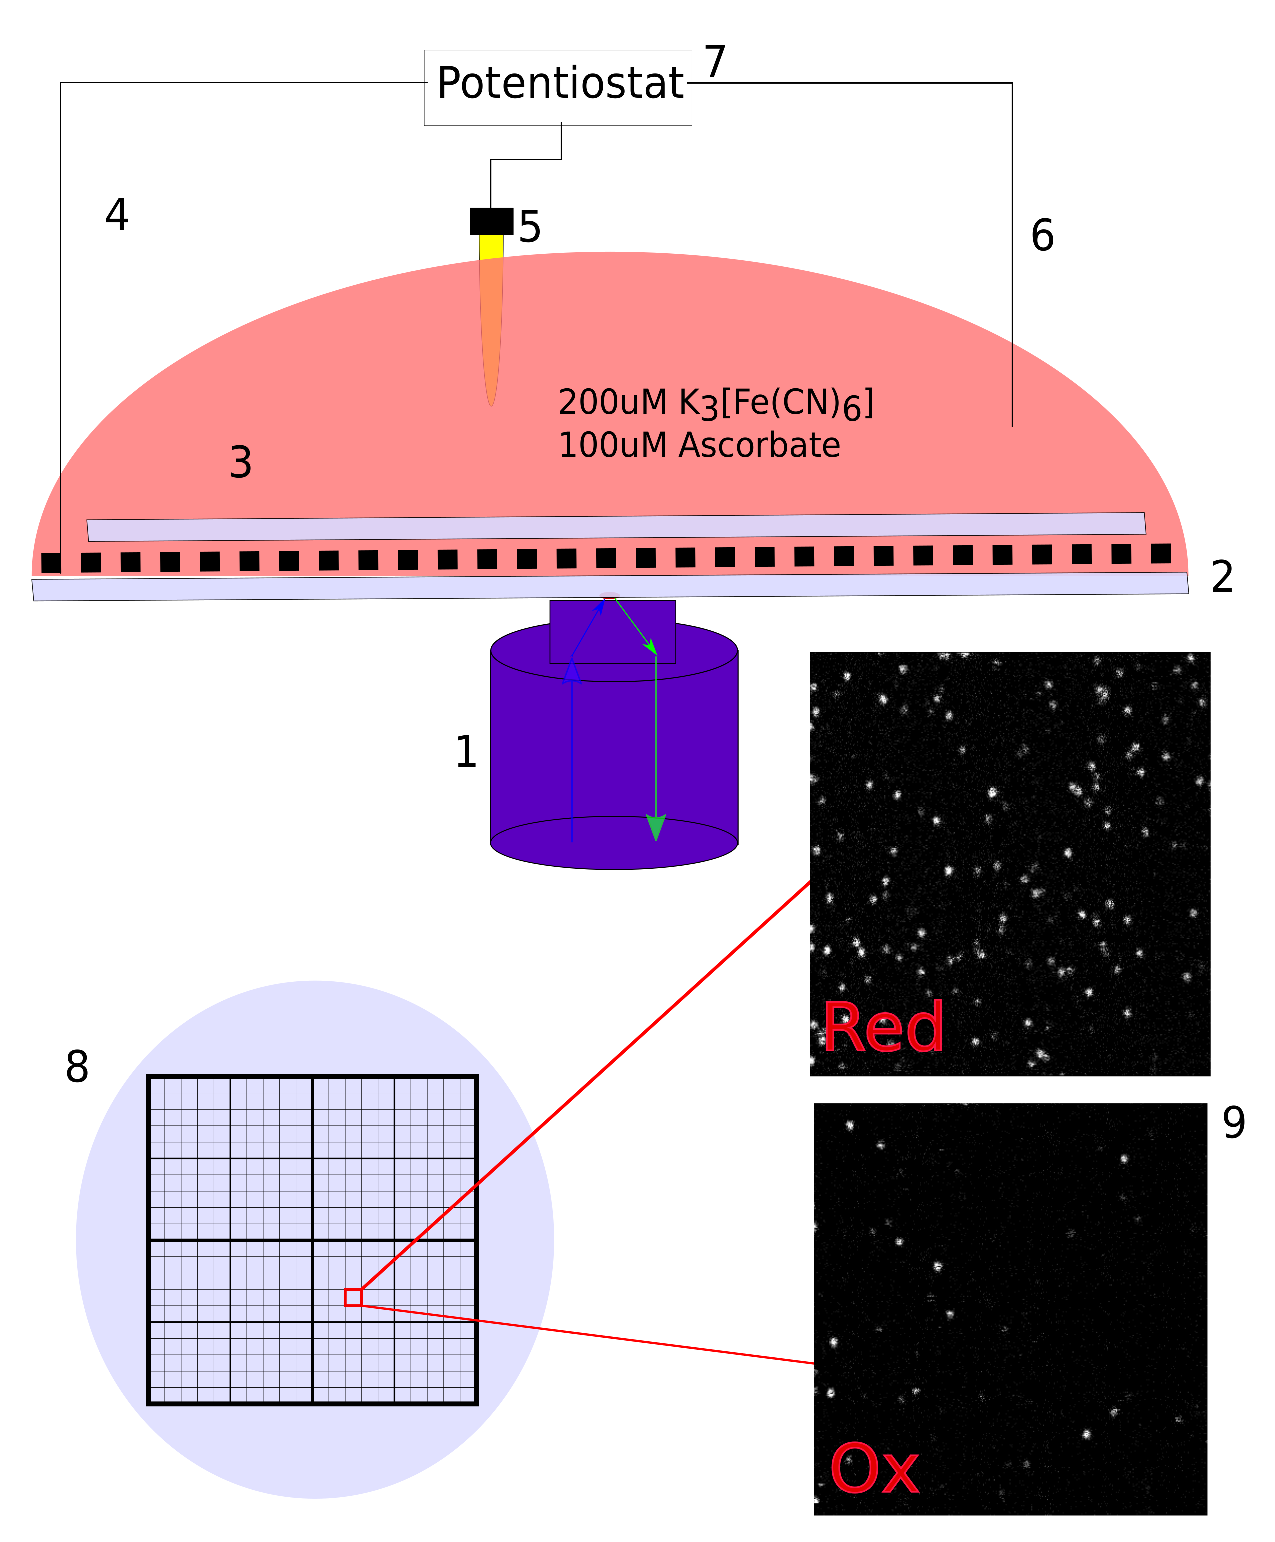
\includegraphics[width=\textwidth]{Figure/Scheme_1_setup.eps}
	The scheme for
	\caption{An example scheme}
  	\label{sch:setup}
\end{scheme}

\begin{figure}
	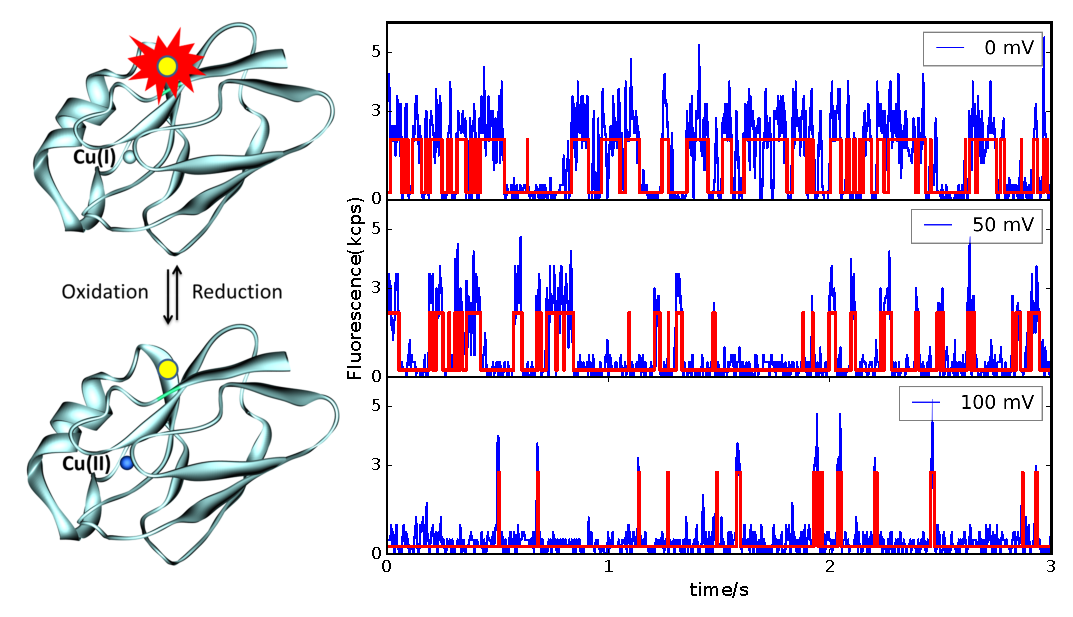
\includegraphics[width=\textwidth]{Figure/Figure_2_timetrace_CuAzu.eps}
	\caption{Time traces of labeled Cu-Azurin at different potential}
	\label{fig:timetrace}
\end{figure}

%%%%%Experimental Section%%%%%%%%%%
\section{Experimental}
\bibliography{Azurin-SMredox}
\end{document}
